\lstset{language=Java,
numberstyle=\footnotesize,
basicstyle=\ttfamily\footnotesize,
frame=shadowbox,
breaklines=true}

\section*{Task 2 - Lucene}

\subsection*{Oppgave a}

Kode lagt til i \textit{MyDocument.java}.
\lstinputlisting[language=Java, firstline=10, lastline=41]{src/ir/MyDocument.java}

\noindent Kode endret i \textit{MyIndexFiles.java}.
\lstinputlisting[language=Java, firstline=21, lastline=41]{src/ir/MyIndexFiles.java}

\noindent Output fra kommandovinduet ved kjøring av \textit{MyIndexFiles.main()} etter modifisering av kode.
\begin{lstlisting}[frame=single]
Usage: java org.apache.lucene.demo.IndexFiles <root_directory>
Indexing to directory 'index'...
adding /Users/hakloev/git/TDT4117/oving4/20news-part/40008
adding /Users/hakloev/git/TDT4117/oving4/20news-part/40027
adding /Users/hakloev/git/TDT4117/oving4/20news-part/40062
... 
for alle 1907 dokumentene
...
adding /Users/hakloev/git/TDT4117/oving4/20news-part/59648
adding /Users/hakloev/git/TDT4117/oving4/20news-part/59652
Optimizing...
1811 total milliseconds

Process finished with exit code 0
\end{lstlisting}

\newpage
\subsection*{Oppgave b}

\subsubsection*{Forklaring av systemet}

\begin{wrapfigure}{r}{0.5\linewidth}
\centering
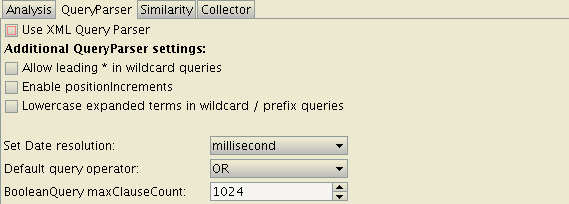
\includegraphics[width=0.4\textwidth]{images/boolean.png}
\caption{QueryParser}
\label{fig:boolean}
\end{wrapfigure}

Luke er et program som bruker indeksene vi genererte med Lucene i forrige oppgave til å vise og modifisere innhold på flere måter.\footnotemark[1] I denne øvingen har vi vært interessert i å sortere etter fire felter: \textit{content, from, path} og  \textit{subject}. Ved å sørge for at Lucene indekserer etter disse feltene, kunne vi generere indeksfiler som kunne brukes i Luke. Vi kunne da søke etter gitte termer i de ulike feltene av dokumentet.\\\hfill

\begin{wrapfigure}{r}{0.5\linewidth}
\centering
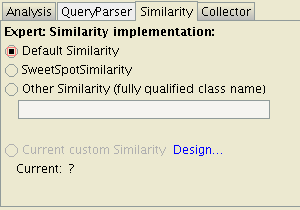
\includegraphics[width=0.5\textwidth]{images/similarity.png}
\caption{Similaritetsmodell}
\label{fig:similarity}
\end{wrapfigure}

Lucene benytter seg av den boolske-modellen til å finne termer i et dokument, og rangerer de med vektor-modellen. Ser vi på figur 1 ser vi at QueryParser er den boolske-modellen og at klausulen er satt til logisk-ELLER. Figur 2 viser at similaritets-modellen er satt til vektor-modellen, da den er ``Default Similarity" i Lucene. Det skal legges til at cosinus-formelen som brukes er modifisert i forhold til den vi har lært faget, men prinsippet er det samme.\footnotemark[2]\\\hfill 

\begin{wrapfigure}{r}{0.5\linewidth}
\centering
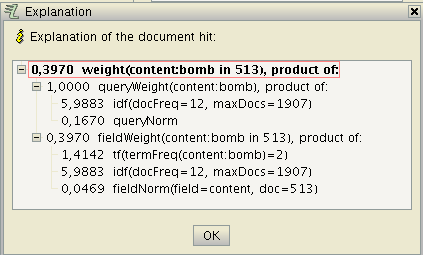
\includegraphics[width=0.5\textwidth]{images/numbers.png}
\caption{Data for dokument 513}
\label{fig:numbers}
\end{wrapfigure}

I figur 3 kan vi se tallene som er til grunn for utregningen av similariteten til dokument 513. Vi ser dokumentet bli rangert til 0,3970, noe som gir plass fem i rangeringen. Dette er fordi rangeringen er produktet av en serie tall, nærmere bestemt produktet mellom spørringsvekt og feltvekt (\textit{query weight} og \textit{field weight}). Her er spørringsvekt igjen et produkt av \textit{idf} (inverse document frequency) og en konstant \textit{queryNorm}. Feltvekt er et produkt av termfrekvens, idf og fieldnorm. Fieldnorm blir regnet ut som følge av lengden på feltet etter stemming, tokanisering og andre operasjoner på dokumentet.  \\\hfill

\footnotetext[1]{https://code.google.com/p/luke/}
\footnotetext[2]{http://lucene.apache.org/core/3\_0\_3/api/core/org/apache/lucene/search/Similarity.html}

\begin{figure}[p]
\centering
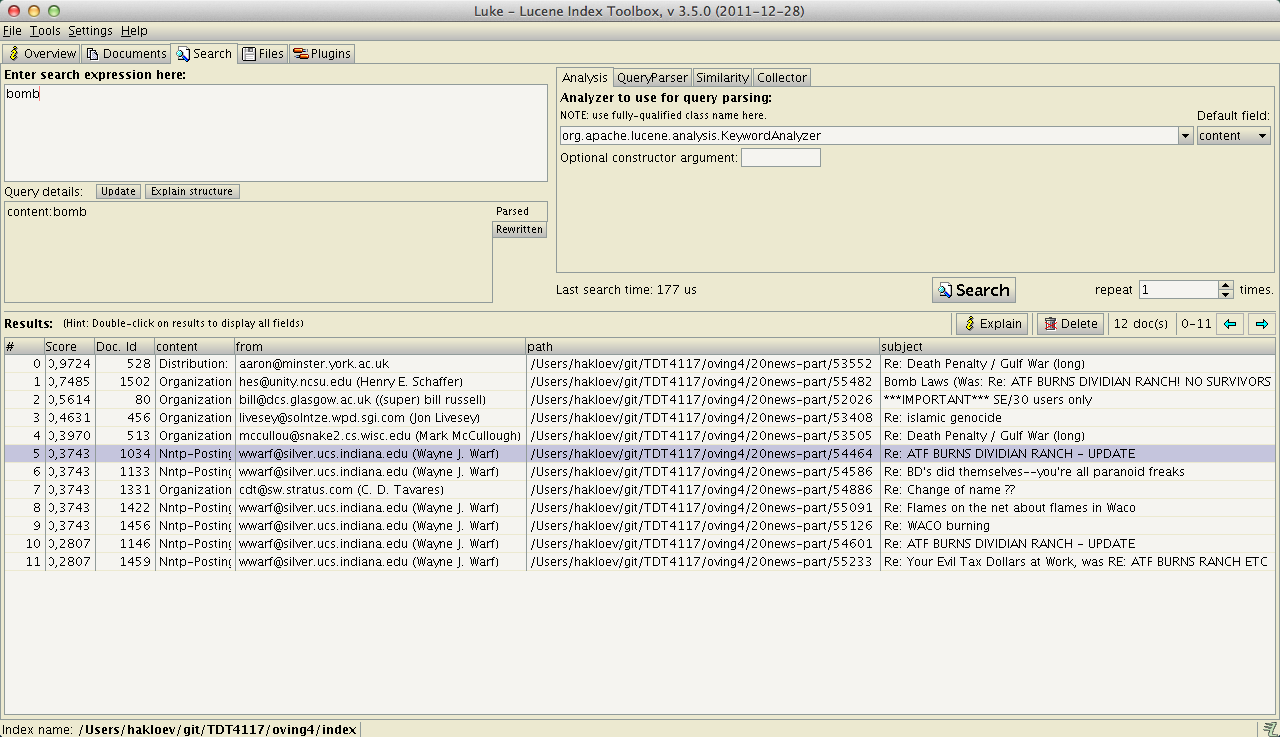
\includegraphics[scale=0.31]{images/bombcontent.png}
\caption{Søk etter bomb i content}
\end{figure}

\begin{figure}[p]
\centering
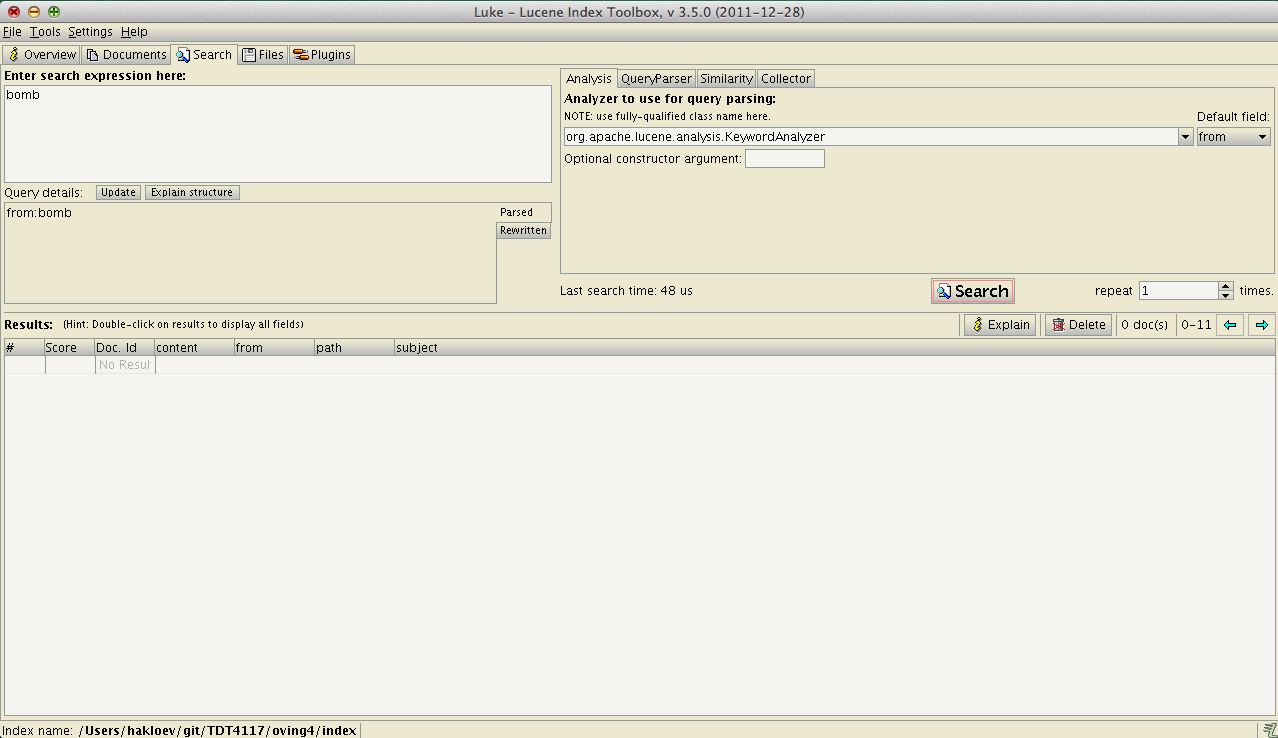
\includegraphics[scale=0.31]{images/bombfrom.png}
\caption{Søk etter bomb i from}
\end{figure}

\begin{figure}[p]
\centering
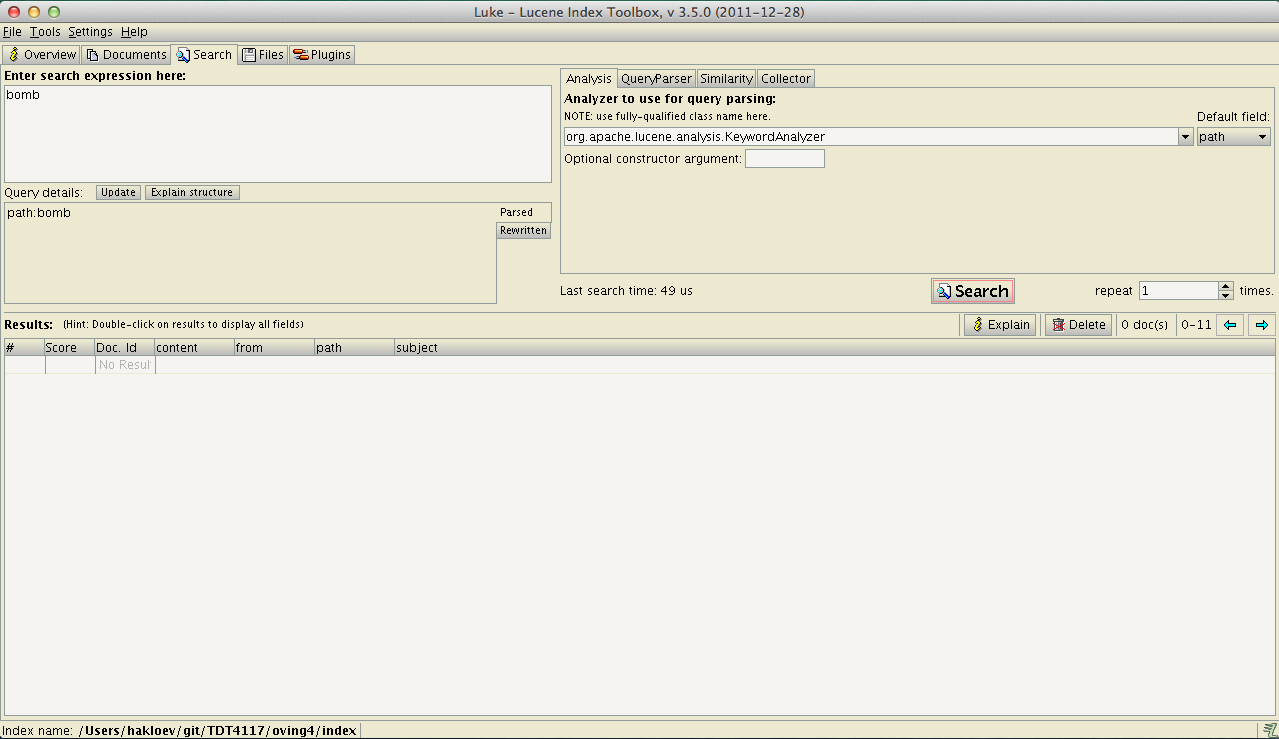
\includegraphics[scale=0.31]{images/bombpath.png}
\caption{Søk etter bomb i path}
\end{figure}

\begin{figure}[p]
\centering
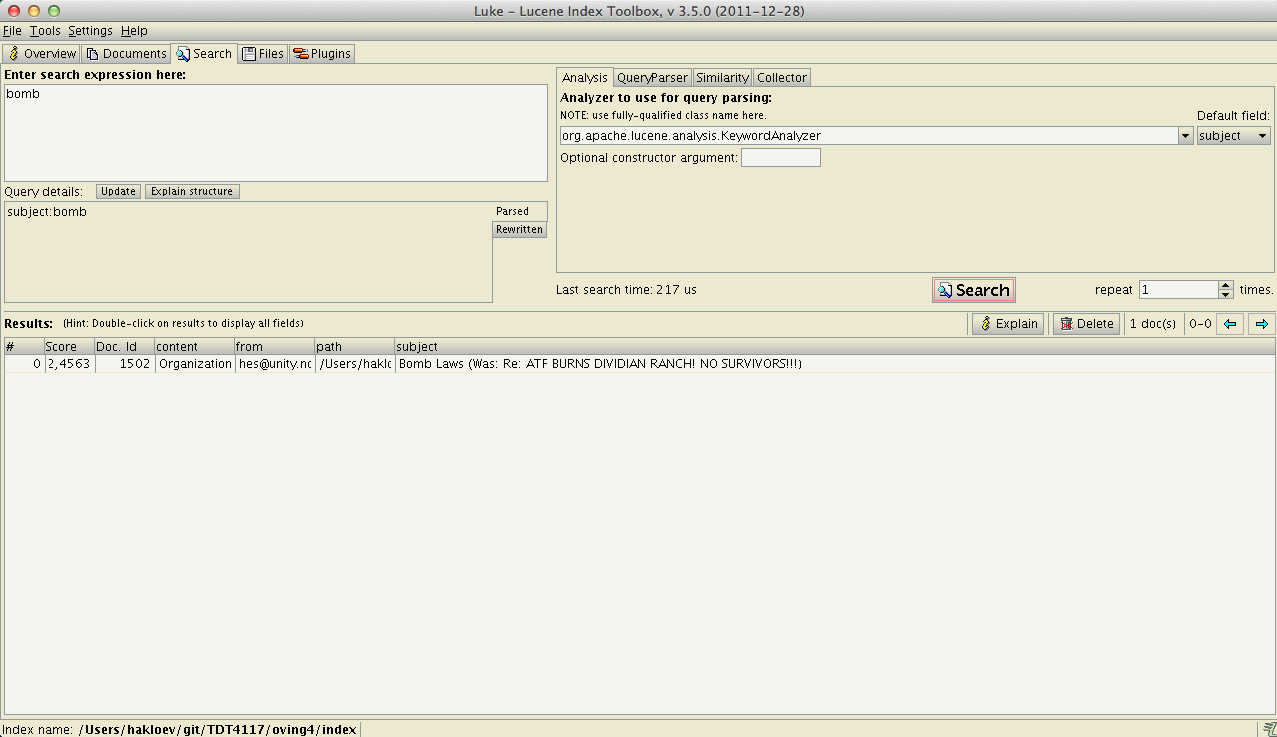
\includegraphics[scale=0.31]{images/bombsubject.png}
\caption{Søk etter bomb i subject}
\end{figure}
